\chapter{Methodology}

\section{Participants}

A total number of \todo{26} participants, \todo{\# females and rest} with the average age of \todo{average age} with the standard deviation of \todo{sd age} took part in the experiment. The participants were all students of the University of Osnabrück. Before the start of the first exploration session all participant gave their written consent for taking part in the experiment (see appx. \ref{appx:forms}, Einverständniserklärung). The participation was voluntary and only students with no health issue were selected (see appx. \ref{appx:forms}, Anamnese). The participants were compensated by test-subject hours and/or 5€ per hour.  

Due to the Covid-19 pandemic sessions were conducted according to the laboratory hygiene regulations with a mask and under 3G rule.

3 participants were excluded due to not being able to comply with the experimental requirements, i.e., come in less than 3 days and more than 4 hours apart.



\section{Experimental Design}

\subsection{City}

This study is conducted in a virtual reality (VR) city with an area of about 1 km\textsuperscript2. The city is consisted of 284 buildings. 56 buildings are used in the experimental task of this study from which 4 are global landmarks, 26 are {\emphasize context meaningful} locations, e.g., shops, construction sites, and 26 are residential, {\emphasize not context meaningful} buildings. These 56 buildings have human agents in front of them and an artwork on one of their walls. Human agents belonging to the shops take the pose of an act according to the functionality of that store {\emphasize(meaningful)}, e.g., has a book in the hand in front of a bookstore, or are just standing in front of the residential building {\emphasize(standing human agent)}. The artworks on the shops are also depicting the functionality of the shop.\\
A sun with a detectable origin is avoided in the city, no street is named and no building is numbered to implicitly direct the participants to prioritize their spatial learning. 

\todo{
	- FIG: include a map \\
	- include photos of the city
}

\subsection{Application and Technology}

The application of the experiment is implemented with unity version 2019.4.11f1. The assets of the city, e.g., buildings, streets were obtained from a previous study called SpaRe, made also at the university of Osnabrück. They were modified with blender version 2.83 LTS (Long Term Support), as were also the human agents picked from Adobe Mixamo collection. They were modified for this experiment in a way that some contextual objects were added to the human agents in front of context meaningful buildings with regard to the context of the building. \\
The experiment consisted of two separate parts, i.e., Exploration and Testing.  Each section had the option to choose the language of the instructions, i.e., German and English. The experiment was conducted using a HTC Vive Pro Eye VR-Headset. For the virtual moving purposes inside the virtual city the participants were given Index valve controller to navigate inside a city by moving the joystick of the controller. They had both the right and left controllers to be able to use their dominant hand.

\section{Experimental Procedure}

Participants were seated on a backless rotating chair that enabled them to physically rotate in the virtual city. Any forward, backward and sideways movement were done utilizing the controllers.

\subsection{Exploration}

The exploration consisted of 5 sessions. The sessions had to be no more than 3 days and no less than 4 hours apart. \\
The total duration of each session was 30 minutes broke down into 10 minutes segments for breaks to reduce the possibility of motion sickness. Before starting each segment the built-in eye-tracker of the VR-Headset was calibrated and validated. \\

After inserting participant-ID and choosing the preferred language the exploration session started with a tutorial. The tutorial was held in a scene separate from the main city. The purpose of the tutorial was to allow the participant to move around, get acquainted with the controller and practice the possible movement options the experiment allowed for. After participants confirmed their confidence in using the controllers the experiment was continued to the exploration session. In the main city participants were advised to explore the city freely.

\subsection{Testing}

Testing comprised of one session of approximately 2 hours. The testing starts after inputting the participant-ID and choosing the language. There is then a tutorial scene outside of the main city used in the experiment for participants to get acquainted with how to use the controller for performing the tasks. Before presenting the trials and in intervals of 112 trials eye-tracker was calibrated and validated. \\

Testing was a pointing task comprised 336 trials performed from 28 different starting locations in the city. The distribution of the starting locations can be seen in figure \ref{fig:starting_locs}. At each starting location 12 target buildings were randomly chosen from a pull of 112 targets (56 task buildings with and without human agents). Some examples are shown in figure \ref{fig:target_photos}. Each of the four conditions of the experiment, i.e., context meaningful with human agent present {\emphasize(CmA)}, context meaningful with no human agent present {\emphasize(CmANo)}, non-context meaningful with human agent present {\emphasize(Sa)}, non-context meaningful with no human agent present {\emphasize(SaNo)} built up 25\% of the trials.  The starting locations themselves were consistent for all participants and their order of execution was randomized for each participant. All movements except the rotation were blocked for the whole testing session to maintain the consistence of the participants' position in the starting locations between participants. \\


\begin{figure}[h]
	\centering
	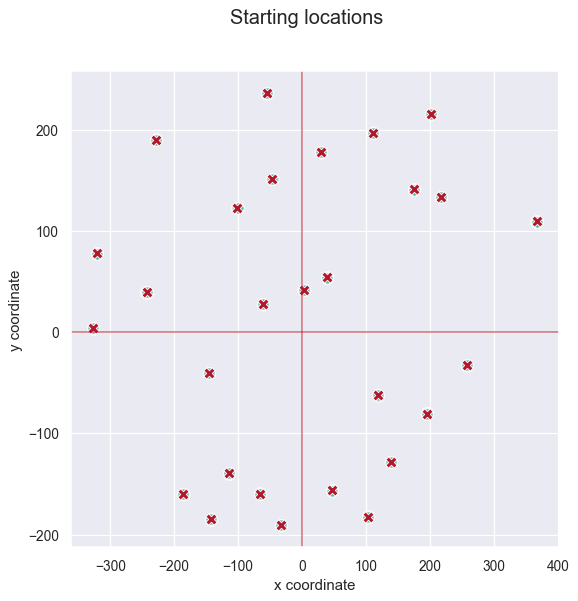
\includegraphics[width=100mm]{figures/starting_locations.png}
	\caption[Distribution of starting locations]{distribution of the starting locations in the city}
	\label{fig:starting_locs}
\end{figure}



\begin{figure}[h!]
	\centering
	\begin{subfigure}[b]{0.48\linewidth}
		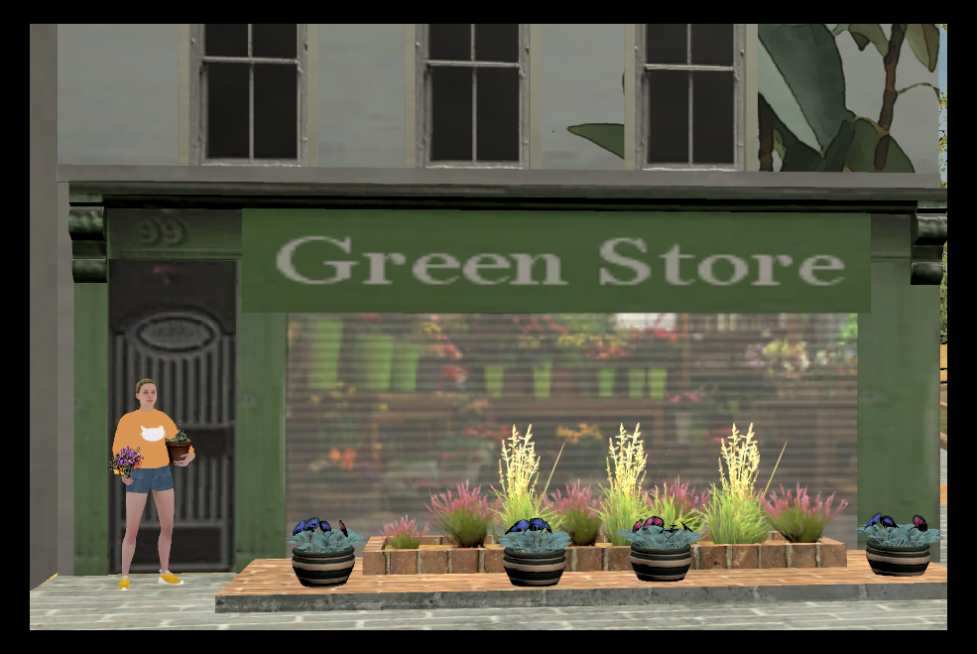
\includegraphics[width=\linewidth]{figures/45_S(green store)_A.PNG}
		\caption{CmA}
	\end{subfigure}
	\begin{subfigure}[b]{0.48\linewidth}
		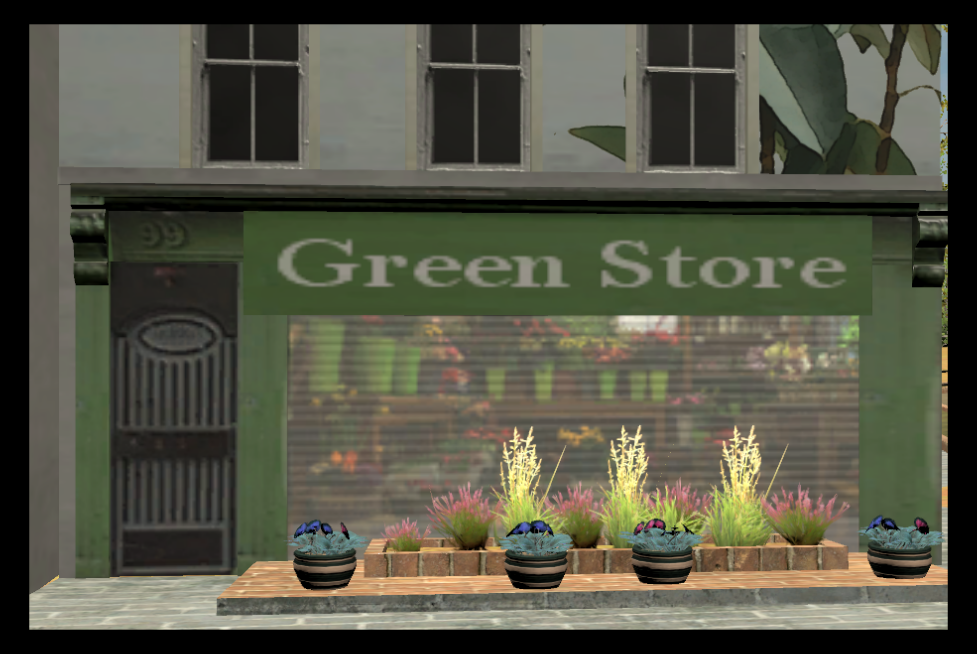
\includegraphics[width=\linewidth]{figures/45_S(green store)_noA.PNG}
		\caption{CmANo}
	\end{subfigure}
	
	
	\begin{subfigure}[b]{0.48\linewidth}
		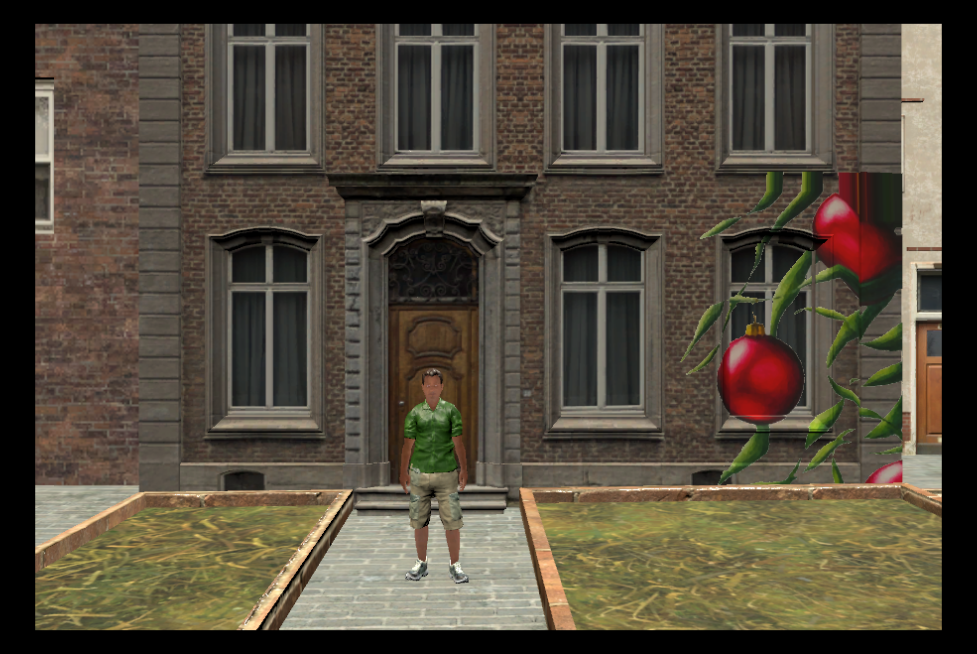
\includegraphics[width=\linewidth]{figures/44_Sa.PNG}
		\caption{Sa}
	\end{subfigure}
	\begin{subfigure}[b]{0.48\linewidth}
		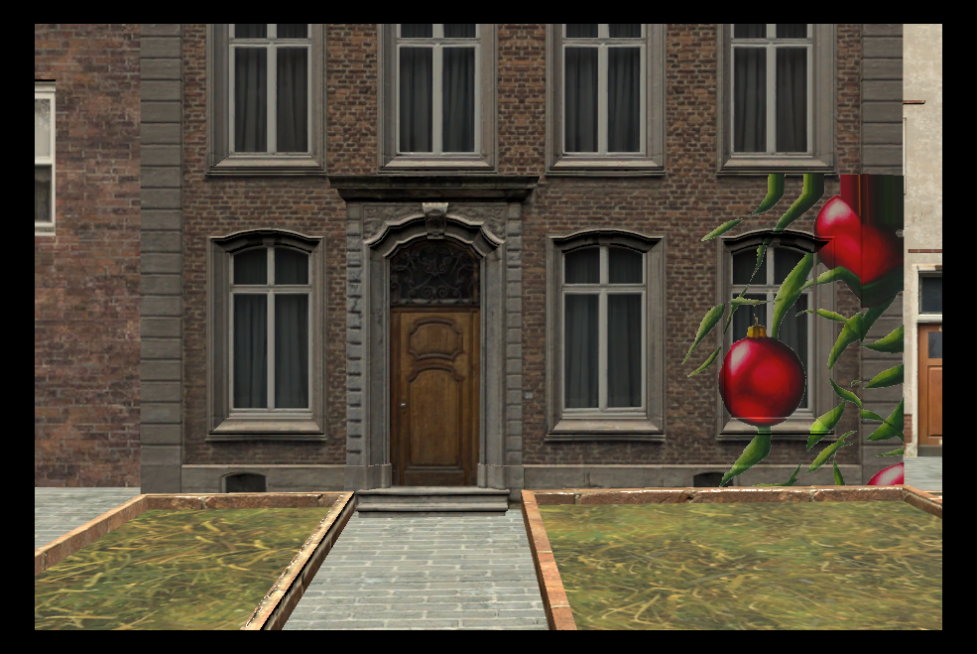
\includegraphics[width=\linewidth]{figures/44_SaNo.PNG}
		\caption{SaNo}
	\end{subfigure}
	

	\caption[Target buildings]{Examples of photos shown in the pointing task as target buildings. A selection of all four experimental conditions.
	\scriptsize{
		\textbf{CmA:}   context meaningful with human agent present.
		\textbf{CmANo:} context meaningful without human agent present.
		\textbf{Sa:}    not context meaningful with human agent present.
		\textbf{SaNo:}  not context meaningful without human agent present.}
}
	\label{fig:target_photos}
\end{figure}


At each starting location the 12 consecutive trials were performed. Before each trial begin a green circular loading bar {\emphasize (Go cue)} was shown in the middle of the screen for 25ms. As soon as the bar was complete, a beep sound was played informing the participants of the start of a new trial. In each trial a photo of one of the task buildings, with or without human agent in front of it (see figure \ref{fig:target_photos}), was presented at the top center of the screen \todo{(see figure X)}. The participants had the option to press the trigger button to bring the picture to the middle of the screen \todo{(see figure X)}. As soon as the button was released the photo moved back to the upper center part of the screen. Since there was no visual virtual body, there was a green dashed laser beam \todo{(see figure X)} attached to the virtual hand of the participants that moved as they moved their hand. The purpose of the laser beam was to assist the participants with the visualization of the direction they are pointing at. The maximum duration of each trial was 30 seconds. If there was no answer given to the task after 20 seconds from the start of the trial, i.e., no direction was selected by the participant indicating in which direction the target building is located from their current location, a countdown timer appeared on the bottom center of the screen \todo{(see figure X)} and terminated the trial after 10 seconds if there was still no answer given. \\

Selecting an answer for the task, i.e., selecting the direction of the target building was possible with a button press. With once pressing the button it locked the laser beam onto a direction and detached it from the hand \todo{maybe a figure of the controller with the info?}. The participants had the option to either confirm the chosen direction with the same button or cancel it with another. Moving on to the next trial was the result of either the participant confirming a direction or by running out of time. Behavioral and technical data, e.g., the chosen direction, participant position and rotation, reaction times were gathered during each trial. The human agents were present during the testing in the city at their exact designated positions and poses in the exploration sessions. A gray screen fade out and fade in occurred while transporting the participants from their current location to another starting location. This was to serve the purpose of decreasing the chance of motion sickness and also avoiding leaking environmental information while moving in the city.

\todo{
	- include photo of the trial  \\
}


\section{Analysis method}

The data of this experiment is gathered from unity in JSON \footnote{Introducing JSON: \href{https://www.json.org/json-en.html}{https://www.json.org/json-en.html}} format. All the further processes for analysis were done in python \autocite{10.5555/1593511} v3.8. For the preprocessing the pandas \autocite{reback2022pandas, mckinney-proc-scipy-2010}, numpy \autocite{harris2020array} and scipy \autocite{2020SciPy-NMeth} libraries, and for the analysis python's statmodels \autocite{seabold2010statsmodels} module were utilized. Matplotlib \autocite{Hunter:2007} and Seaborn \autocite{Waskom2021} were used for the visualizations.\\

After importing and converting the data into a pandas dataframe, the preprocessing is done to prepare the data for analysis. In this process the dependent variable {\emphasize absolute\_180\_angle} is derived. The variable contains the absolute angular deviation of the participant's chosen direction from the actual target position. 

\subsection{Preprocessing}

Different functions of pandas {\emphasize (pd)} and numpy {\emphasize (np)} used for the preprocessing. In all the calculations involving directions and positions, only the right direction (x) and the forward direction (z) are taken into account. The up direction (y) was excluded as it is not relevant for the analysis at hand. \\

The main preprocessing steps are as follow:

\begin{enumerate}
	\item Removed trials in which the participants did not select any direction. These were the trials that were terminated due to timeout. Hence, only the trials where their respective TimeOut variable was False were kept for the analysis. \\
	
	\item Calculated the participant's chosen direction's absolute angular deviation from the actual location of the target building.
	
	\begin{enumerate}
		%\item Calculating the absolute Euclidean distance between the participant’s position and the target building. 
		\item Translated the target building's center position {\emphasize(Tpos)} by the participant's body position {\emphasize(Ppos)} to be able to derive the translated building center position {\emph{Tpos\_t}} take the body position as the origin at the (0,0) coordinates.
		
			\begin{align*}
				Tpos\_t_{x,z}= Tpos_{x,z} - Ppos_{x,z}
			\end{align*}
		
		The direction vector of participant's chosen direction doesn't need to be translated because unity's output for a direction is a normalized vector and therefore it's origin lies already at (0,0).\\
		
		\item Now that body position is at (0,0) with respect to the translated building center position, the angle difference between the participant's chosen direction {\emphasize(Cdir)} to the positive x-axis and the translated building center position {\emphasize(Tpos\_t)} to the positive x-axis were calculated using numpy arctan2(z, x) \footnote{Numpy arctan2: \href{https://numpy.org/doc/stable/reference/generated/numpy.arctan2.html}{https://numpy.org/doc/stable/reference/generated/numpy.arctan2.html}} function. This function calculates the angle in radian between the positive x-axis and the vector given to the function as parameter. \\
		Due to the translation done in step \emph{a} the body position was implicitly translated to the origin (0,0), i.e., subtracting body position from body position results in (0,0), it was possible to pass the z and x coordinates of the {\emphasize Tpos\_t} and the {\emphasize Cdir} to the arctan2 function separately to calculate the angle between the {\emphasize Cdir} and the positive x-axis {\emphasize (Cdir\_to\_x)} and the {\emphasize Tpos\_t} and the positive x-axis {\emphasize (Tpos\_to\_x)}. The results are directly translated to degree utilizing numpy rad2deg() \footnote{Numpy rad2deg: \href{https://numpy.org/doc/stable/reference/generated/numpy.rad2deg.html}{https://numpy.org/doc/stable/reference/generated/numpy.rad2deg.html}} function.
	
		\begin{align*}
			Tpos\_to\_x_{\theta} & = np.rad2deg(np.arctan2(Tpos\_t_{z}, Tpos\_t_{x})) \\
			Cdir\_to\_x_{\theta} & = np.rad2deg(np.arctan2(Cdir_{z}, Cdir_{x}))
		\end{align*}
		
		\item After creating {\emphasize Tpos\_to\_x} and {\emphasize Cdir\_to\_x} the angles were respectively converted to {\emphasize Tpos\_to\_x\_360} and {\emphasize Cdir\_to\_x\_360} in the 360 degree environment.

		\begin{align*}
			Tpos\_to\_x\_360_{\theta} = & \\
			& if & \\
			&& Tpos\_to\_x_{\theta} < 180 \\
			& then & \\
			&& 360 + Tpos\_to\_x_{\theta} \\
			& else & \\
			&& Tpos\_to\_x_{\theta}
		\end{align*}
	
		\begin{align*}
			Cdir\_to\_x\_360_{\theta} = & \\
			& if & \\
			&& Cdir\_to\_x_{\theta} < 180 \\
			& then & \\
			&& 360 + Cdir\_to\_x_{\theta} \\
			& else & \\
			&& Cdir\_to\_x_{\theta}
		\end{align*}
		
		\item Calculated the angular difference between the selected direction {\emphasize (Cdir\_to\_x\_360)} and the target building {\emphasize (Tpos\_to\_x\_360)}. They were directly converted to the signed 2 quadrant environment.
		
		\begin{align*}
			signed\_180\_angles_{\theta} = ((Tpos\_to\_x\_360_{\theta} - Cdir\_to\_x\_360_{\theta}) + 180) \% 360 - 180
		\end{align*}
	
		\item The final step was to create {\emphasize absolute\_180\_angles}, the dependant variable for the main analysis in LMM. This variable stores the absolute value of the angular differences contained in {\emphasize signed\_180\_angles}. The reason for using absolute values is that the direction of the deviation is not a deciding factor in how accurate the participants performed the pointing task. Taking the absolute values is done with numpy abs() \footnote{Numpy absolute: \href{https://numpy.org/doc/stable/reference/generated/numpy.absolute.html}{https://numpy.org/doc/stable/reference/generated/numpy.absolute.html}} function.
		
		\begin{align*}
			absolute\_180\_angles_{\theta} = np.abs(signed\_180\_angles_{\theta})
		\end{align*}
		
	\end{enumerate}

	\item Calculated the Euclidean distance from the participant's body position to the target building for each trial. This was done using the Euclidean distance function \footnote{Scipy spatial Euclidean distance: \href{https://docs.scipy.org/doc/scipy-1.8.0/reference/generated/scipy.spatial.distance.euclidean.html\#scipy.spatial.distance.euclidean}{https://docs.scipy.org/doc/scipy-1.8.0/reference/generated/scipy.spatial.distance.euclidean.html\#scipy.spatial.distance.euclidean}} of scipy spatial.
	
	\begin{align*}
		body\_to\_target_{dis} = Euclidean\_distance((Ppos_x, Ppos_z), (Tpos_x, Tpos_z))
	\end{align*}

\end{enumerate}



\subsection{Analysis}
Due to the hierarchical structure of the data, Linear Mixed Models (LMM) were chosen as the method of analysis. For that the python's statmodels module were used.

\subsubsection{Dependent variables}

\begin{enumerate}
	\item \textbf{Absolute angular deviation} {\emphasize (absolute\_180\_angles)}: the absolute value of the angular deviation of the direction chosen by the participant from the actual location of the target building shown at each trial. This variable has the mean of 48.08 with the standard deviation of 44.30, and median of 33.70. (See figure \ref{fig:angular_dev_dists})
	
	
	\begin{figure}[h]
		\centering
		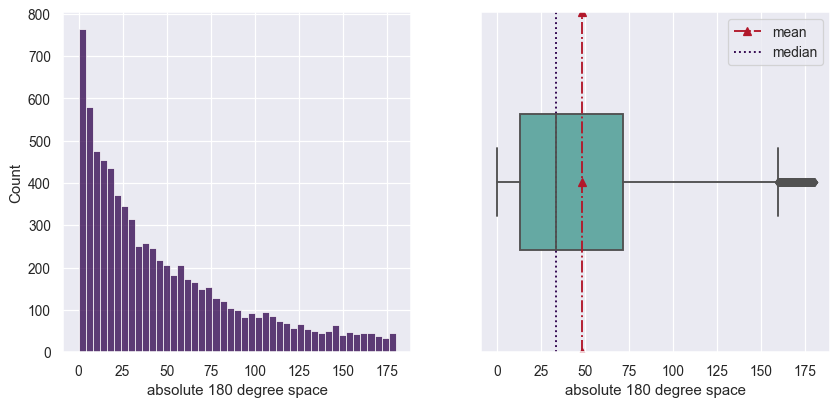
\includegraphics[width=150mm]{figures/angular_deviation_hist_box_23.png}
		\caption[Distribution of the absolute angular deviation]{distribution of the absolute angular deviation}
		\label{fig:angular_dev_dists}
	\end{figure}

	\item \textbf{Reaction times} {\emphasize (RT)}: this variable stores the duration between start of each trial and the time the participants confirmed a direction as their respond. The begin timestamp of the trial is directly after the go cue is completed and the end timestamp instantly after the response is given. Calculating the duration is done in unity. This variable has the mean of 7.77 with the standard deviation of 5.56, and median of 6.06. (See figure \ref{fig:rt_dists})
	
	\begin{align*}
		RT = end\_timestamp - begin\_timestamp
	\end{align*}

	\begin{figure}[h]
	\centering
	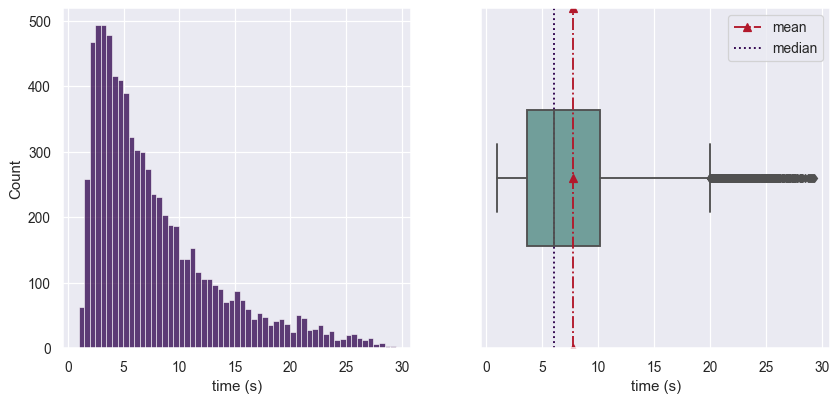
\includegraphics[width=150mm]{figures/RT_hist_box_23.png}
	\caption[Distribution of reaction times]{distribution of the  reaction times in the pointing task}
	\label{fig:rt_dists}
\end{figure}

\end{enumerate}

\subsubsection{Independent variables}

\begin{enumerate}
	\item \textbf{Starting locations:} the 28 different starting locations spread out through the city. See the full list of the locations in appx. \ref{appx:starting_locations}. \\
	
	\item \textbf{Distance to the target:} this variable is the distance of the participant to the target building at each starting location.
\end{enumerate}

